\chapter{Survey Results}
\label{survey_results}

\begin{center}
  \hspace*{-1.9cm}
  \begin{tabular}{ p{8.7cm} p{8.7cm} }
  	\textbf{Questions Related to MicroNet and Java} & 
  	(ascending grades; 1 worst, 5 best) \\[1cm]
  
    Do you rate Java as a good solution to achieve application platform
    independence? &
    How do you rate the acceptance of Java in the software industry?\\
    
    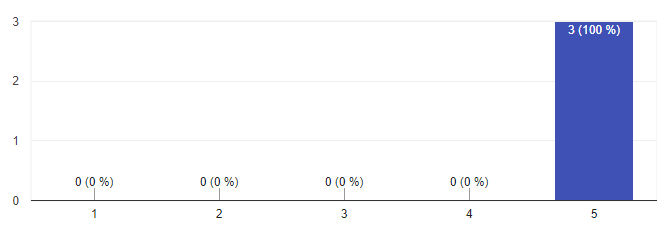
\includegraphics[width=\linewidth]{images/survey/java1}
    &
    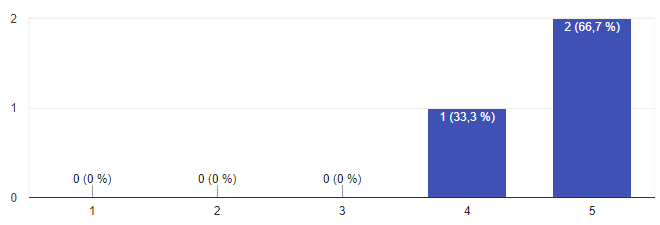
\includegraphics[width=\linewidth]{images/survey/java2}\\[1cm]
    
    How do you rate the suitability of modern Java features like annotation
    processing, code generation, and functional programming (Lambdas) to
    implement composition concepts for distributed applications? & 
    Do you think using Maven as the main driver to define versioning and the
    build process of an application is a good solution?\\
    
    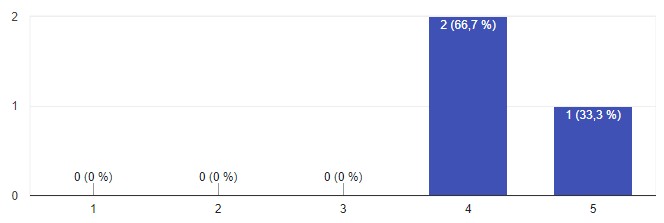
\includegraphics[width=\linewidth]{images/survey/java3}
    &
    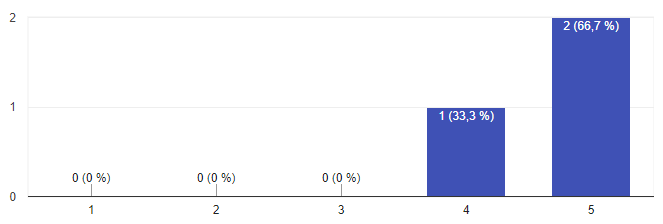
\includegraphics[width=\linewidth]{images/survey/java4}\\[1cm]
    
    Do you find the predefined (very directory heavy) Maven project structure
    cumbersome? & \\
    
    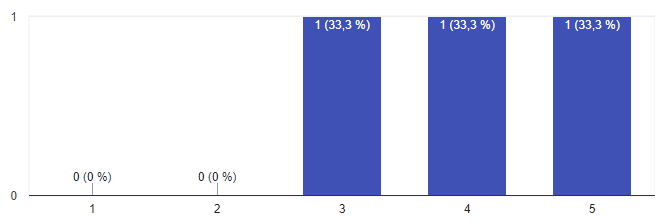
\includegraphics[width=\linewidth]{images/survey/java5}
    & \\
  \end{tabular}
\end{center}


\begin{center}
  	\hspace*{-1.9cm}
  	\begin{tabular}{ p{8.7cm} p{8.7cm} }
  
    	\textbf{Questions Related to Distributed Application Design} & 
  		(ascending grades; 1 worst, 5 best) \\[1cm]
  		
  		Did MicroNet help you to understand the challenges that distributed
  		application design introduces? &
  		How do you rate the \textit{Shared Model} approach which is used to
  		distribute the application's domain model among Microservices?\\
      	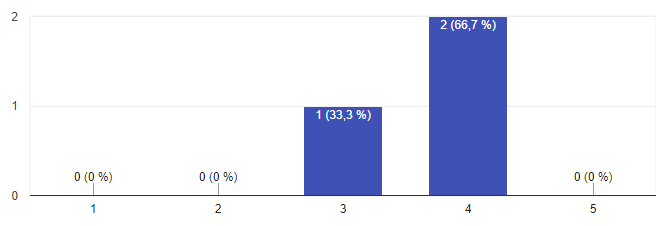
\includegraphics[width=\linewidth]{images/survey/app1}
    	&
    	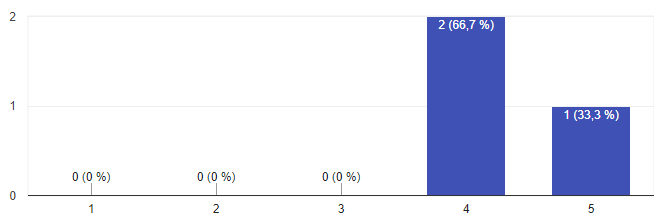
\includegraphics[width=\linewidth]{images/survey/app2}\\[1cm]
    	
    	What do you think about the overhead introduced by documenting the
    	\textit{Shared API} with Java annotations? &
    	Is the presentation of the \textit{Shared API} to the developer through
    	\textit{Code Assist} a helpful contribution to \ms{} composition?\\
    	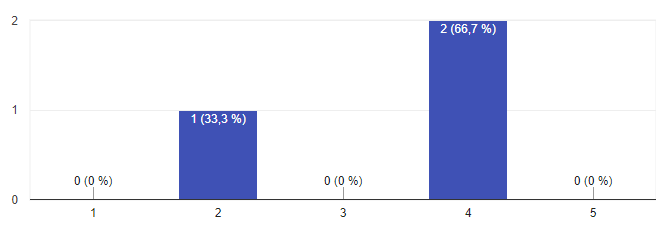
\includegraphics[width=\linewidth]{images/survey/app3}
    	&
    	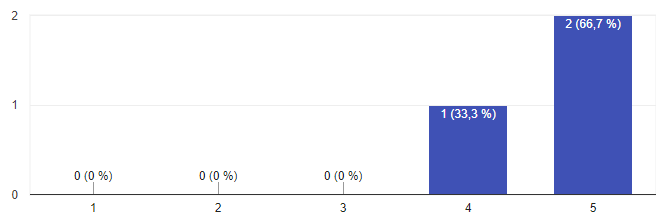
\includegraphics[width=\linewidth]{images/survey/app4}\\[1cm]
    	
    	Do the \textit{Launch Utilities} offered by the \textit{Service Explorer}
    	help with building and deploying \ms{} applications? & \\
    	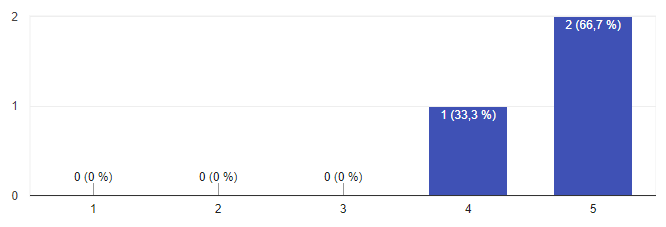
\includegraphics[width=\linewidth]{images/survey/app5}
    	& \\
    \end{tabular}
\end{center}

\textbf{Additional Comments to Distributed Application Design:}

\begin{itemize}
  \item \textit{``Being strictly pro in-code documentation I like the idea with
  the annotations. However, lots of the information provided there can be
  automatically derived from the code. This introduces unnecessary boilerplate
  and after changing a service multiple times during development, the
  annotations are most-likely no longer in-sync with the actual
  implementation.''}
  \item \textit{``The service explorer is also quite helpful. Nonetheless, after
  having published (or started) a service as a container once, it can no longer be
  done using the service explorer (it will end in a name conflict since the
  plugin tries to create a new container instance). Therefore, it would be handy
  if the service/container with the same name is either (re)started or
  overwritten if changes were made (of course, with confirmation).''}
\end{itemize}

\begin{center}
  	\hspace*{-1.9cm}
  	\begin{tabular}{ p{8.7cm} p{8.7cm} }
  
    	\textbf{Questions Related to MicroNet Respecting the \msuc{} Tenets} & 
  		(ascending grades; 1 worst, 5 best) \\[.7cm]
  		
  		Fine-grained Interfaces and Single Responsibility &
		Domain-Driven-Design\\
		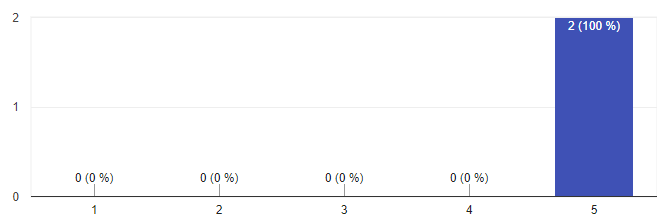
\includegraphics[width=\linewidth]{images/survey/tenet1}
    	&
    	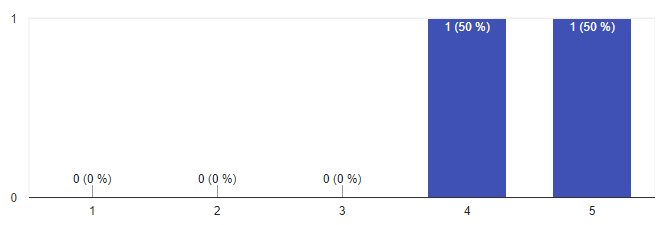
\includegraphics[width=\linewidth]{images/survey/tenet2}\\[.7cm]

		IDEAL &
		Polyglot Programming and Persistence\\
		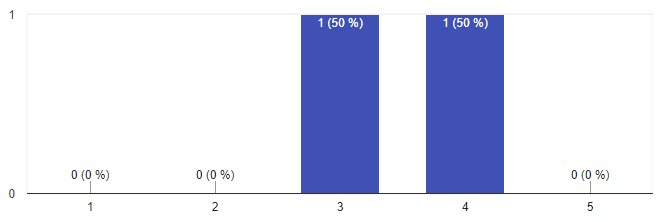
\includegraphics[width=\linewidth]{images/survey/tenet3}
    	&
    	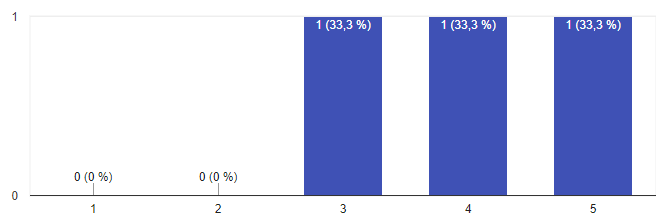
\includegraphics[width=\linewidth]{images/survey/tenet4}\\[.7cm]
		
		Lightweight Containers &
		Decentralized Continuous Delivery\\
		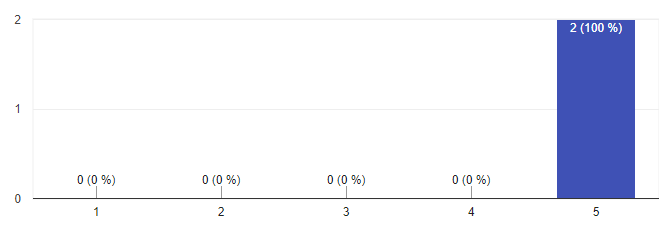
\includegraphics[width=\linewidth]{images/survey/tenet5}
    	&
    	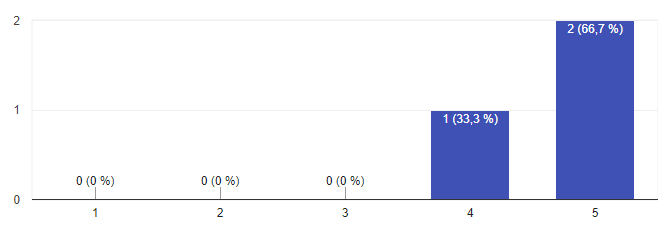
\includegraphics[width=\linewidth]{images/survey/tenet6}\\[.7cm]
		
		DevOps & \\
		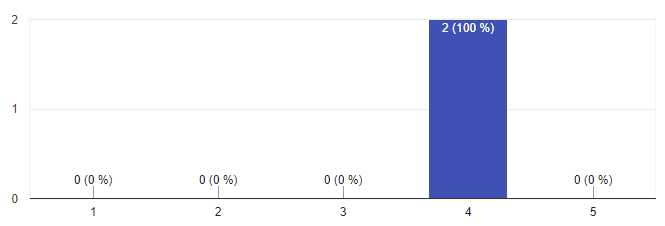
\includegraphics[width=\linewidth]{images/survey/tenet7}
    	& \\
    \end{tabular}
\end{center}

\textbf{Additional Comments to \msuc{} Tenets:}

\begin{itemize}
  \item IDEAL
  \begin{itemize}
    \item \textit{``While the services themselves appear to respect this approach,
    I think it is violated by the use of the relational database PostgreSQL (in AccountDB).
	However, it is used as an example application and no-one is forced to use it.
	Nevertheless, I believe examples should reflect the scenarios in the best
	possible way.''}
	\item \textit{``Also, this relational database can be a single point of failure.
	Furthermore, how do the relying services (at least in the example) react if the
	database crashes. I feel they will fail as well as in the tutorial it is
	already noted that the order the services are started is essential. In my
	opinion also a violation of the \ms{} principle for both, the providing
	and the using services.''}
  \end{itemize}
  \item DevOps
   \begin{itemize}
    \item \textit{``Also problematic by the use of the relational database.''}
   \end{itemize}
\end{itemize}

\begin{center}
  	\hspace*{-1.9cm}
  	\begin{tabular}{ p{8.7cm} p{8.7cm} }
  
    	\textbf{Questions About MicroNet in General} & 
    	(ascending grades; 1 worst, 5 best) \\[1cm]
    	
    	How easy was it to install MicroNet? &
    	How user-friendly is the graphical user interface (Eclipse Views) of
    	MicroNet?\\
    	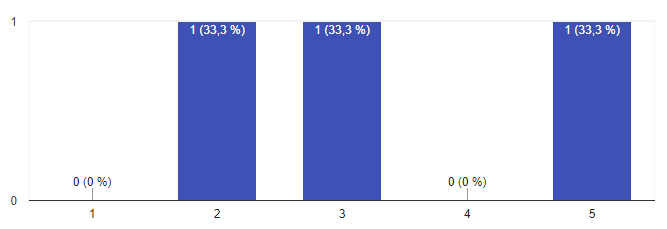
\includegraphics[width=\linewidth]{images/survey/mn1}
    	&
    	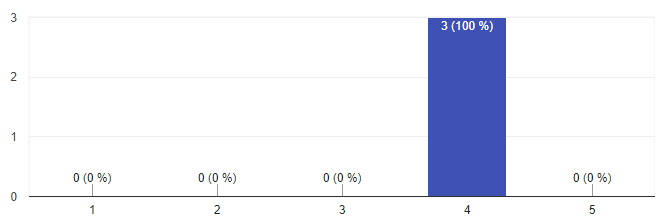
\includegraphics[width=\linewidth]{images/survey/mn2}\\[1cm]
    	
    	How often did you encounter freezes or crashes? &
    	Did you experience system behavior that you did not understand like
    	messages or error logs?\\
    	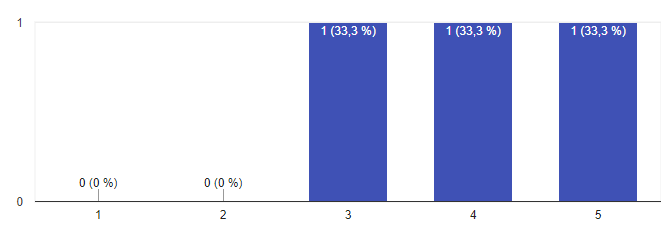
\includegraphics[width=\linewidth]{images/survey/mn3}
    	&
    	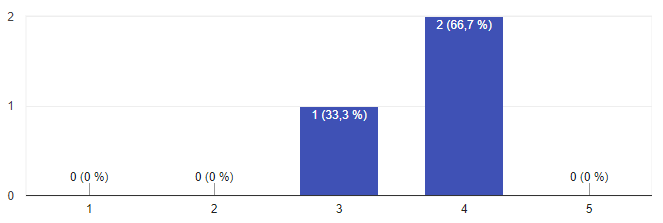
\includegraphics[width=\linewidth]{images/survey/mn4}\\[1cm]
    	
    \end{tabular}
    \hspace*{-1.9cm}
  	\begin{tabular}{ p{8.7cm} p{8.7cm} }
    	What is your overall feeling about the performance of MicroNet? &
    	How likely are you to recommend MicroNet to others? \\
    	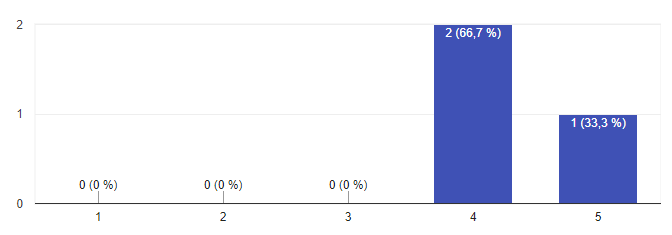
\includegraphics[width=\linewidth]{images/survey/mn5}
    	&
    	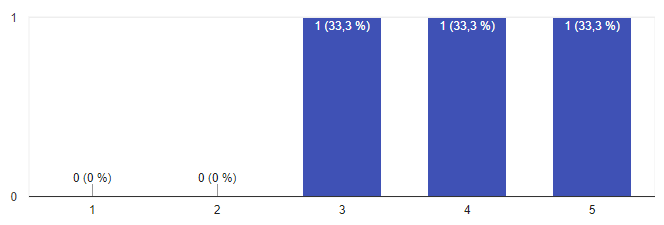
\includegraphics[width=\linewidth]{images/survey/mn7}\\[1cm]
    	
    \end{tabular}
\end{center}

\begin{center}
	\hspace*{-1.9cm}
  	\begin{tabular}{ p{17.4cm} }
  	Which areas of MicroNet need to be improved the most? \\
  	
  	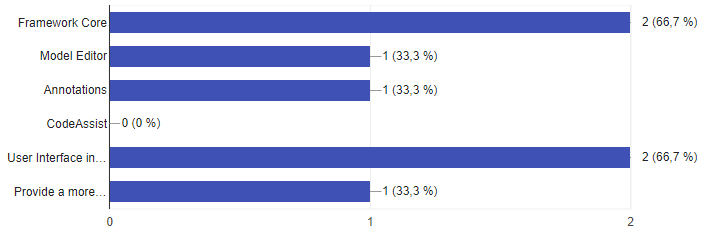
\includegraphics[width=\linewidth]{images/survey/mn6}
    \\
  	
  	\end{tabular}
\end{center}

\begin{center}
	\hspace*{-1.9cm}
  	\begin{tabular}{ p{17.4cm} }
  	\textbf{Background of the Survey Participants:}
  	
  	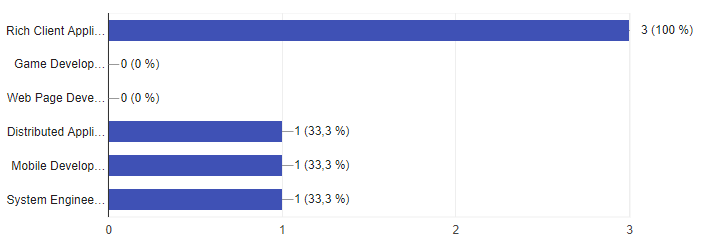
\includegraphics[width=\linewidth]{images/survey/experience}
    \\
  	
  	\end{tabular}
\end{center}

\section*{Additional Comments to MicroNet}

\begin{itemize}
  \item \textit{``It appears to grow into an interesting product. But I have the
  feeling that MicroNet is unnecessarily concentrated on the gaming topic. Most
  of the things are barely related to gaming (if not only the examples) and can
  be surely used in other fields quite nicely. Thus, I suggest to extract the
  gaming parts into a separate (sub-) project, or at least not only aiming to be
  a framework for the game development.''}
  \item \textit{``After a few small adjustments in the installation and
  configuration process, the framework is quite easy to use. It would be
  interesting to see other examples than games.''}
  \item \textit{``Performance is hard to criticize on this small setup.
  Hopefully some graphs illustrating the performance will be presented.''}
  \item Framework Core
  \begin{itemize}
    \item \textit{``Does the "timing relevancy" not violate the
    scalability/micro-service model?''}
    \item \textit{``Meaning that certain services have to be started prior
    others, what happens if one of these crashes/needs to be restarted?''}
  \end{itemize}
  
  \item Model Editor
  \begin{itemize}
    \item \textit{``Provide the possibility to document the models. It feels
    inconsistent if only the services can be documented.''}
  \end{itemize}
  
  \item Annotations
  \begin{itemize}
    \item \textit{``As already stated earlier, the documentation annotations are
    interesting, but since most information can derived from the code they are boilerplate.''}
  \end{itemize}
  \item User Interface in General
  \begin{itemize}
    \item \textit{``As the user interface provides quite a bunch of different
    views, I suggest providing a custom perspective.''}
    \item \textit{`` Settings page: "Test Network" gets a "succesful" tick even
    nothing is entered (and the test obviously fails)''}
    \item \textit{``Account Service: Is it really a good idea deciding on the
    project's name if the additional projects should be created?''}
  \end{itemize}
  
\end{itemize}



